\section{Testing}
The scenario used for testing is the one shown in figure \ref{fig:threestationsetup}.\\
Each station sends a message that looks like this:
\begin{align*}
Packet &= S to R\\
S &= ThisStation\\
R &= neighbours[receiver].stationID
\end{align*}

Where Packet is the packet that is sent to the receiver, S is the station ID of the sending station and R is the station ID of the receiving station.\\
For example, for station 1 sending to station 3: $1\ to\ 3$\\
\\~
%Screenshot of testing this for three stations, where all stations sends one message to each of the other two:
The test was made with the three stations and an error frequency of 90\% (command: ./network -pmynetwork -e900 -n3). This test was run multiple times to reduce the possibility of lucky streaks.
\begin{figure}[H]
\centering
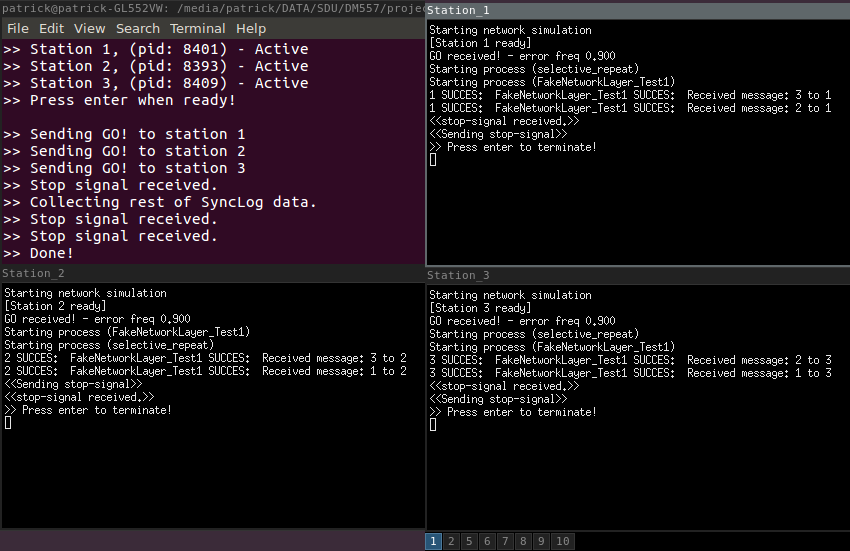
\includegraphics[width=\textwidth]{Test3.png}
\caption{Test of three stations, each sending a message to the other two}
\label{fig:threestationtest}
\end{figure}

As seen in figure \ref{fig:threestationtest}, the three stations each received two messages, one from each of the other two stations.



